\chapter{Introduction to linear regression}
\label{linRegrForTwoVar}


	For data that seems to have a nonlinear trend, we can often transform the variables to obtain a linear trend.
	Linear relationships have the pleasing feature that the correlation coefficient $\rho=\rho_{X,Y}$ is $\pm 1$ exactly when
	there is a perfect linear relationship between the variables $X$ and $Y$\footnote{
		A similar result for, say, quadratic or exponential relationships is not known to us.
	}.

\section{Deriving formulas for linear regression}
	We seek that values $b_0$, $b_1$ that minimize the sum of squared errors $(y_i-(b_0+b_1x_i))^2$.
	So we take the derivatives with respect to $b_0$ and $b_1$ and set them equal to zero.
	For fixed $b_1$, let
	\[
		f(b_0) = \sum_{i=1}^n (y_i-(b_0+b_1x_i))^2
	\]
	and let us solve
	\[
		0 = f'(b_0) = -2 \sum_{i=1}^n (y_i-(b_0+b_1x_i))
	\]
	Dividing by $-2n$,
	\[
		0 = \overline y - b_0 - b_1\overline x
	\]
	which means $\overline y = b_0+b_1\overline x$.
	In other words, the point of means $(\overline x,\overline y)$ lies on the regression line.
	Now for fixed $b_0$, we want to solve for $b_1$.
	It will be useful to use the notations
	\begin{eqnarray*}
	\overline{xy}  &=& \frac1n\sum_{i=1}^nx_iy_i,\quad\text{ and}\\
	\overline{x^2}&=& \frac1n\sum_{i=1}^nx_i^2
	\end{eqnarray*}
	Let
	\[
		g(b_1) = \sum_{i=1}^n (y_i-(b_0+b_1x_i))^2
	\]
	Setting the derivative equal to zero:
	\begin{eqnarray*}
		0 &=& g'(b_1) = -2 \sum_{i=1}^n (y_i-(b_0+b_1x_i))(x_i)\\
		0 &=& \overline{xy} - b_0\overline x - b_1\overline{x^2}\\
		0 &=& \overline{xy} - (\overline y-b_1\overline x)\overline x - b_1\overline{x^2}\\
		0 &=& \overline{xy} - (\overline y\cdot \overline x)+b_1[(\overline x)^2 - \overline{x^2}]
	\end{eqnarray*}
	\begin{equation}\label{b1}
		b_1 = \frac{\overline{xy} - \overline x\cdot\overline y}{\overline{x^2}-(\overline x)^2}.
	\end{equation}

	%\textC{\newpage}

	As taught in Calculus III, this is the beginning of the process of finding a maximum.
	Let us compare our value of $b_1$ to that stated in \emph{OpenIntro Statistics}:
	\begin{equation}
		b_1 \overset{!}{=} \frac1{n-1}\sum (x_i-\overline x)(y_i-\overline y)/s_x^2
		= \frac{\sum (x_i-\overline x)(y_i-\overline y)}{\sum_{i=1}^n (x_i-\overline x)^2}
	\end{equation}
	and we see that our calculation is correct.

	\index{linear regression|textbf}

	Let us furthermore compare this to the correlation coefficient $r$.
	We shall have\footnote{
		In \emph{OpenIntro Statistics}, the symbol $R$ is used, but we shall use $r$.
		See \url{https://stats.stackexchange.com/questions/134167/is-there-any-difference-between-r2-and-r2} for a discussion of this issue.
	}
	\[
		b_1=r s_y/s_x.
	\]
	In other words,
	\[
		r = \frac{\sum (x_i-\overline x)(y_i-\overline y)}{\sqrt{\sum_{i=1}^n (x_i-\overline x)^2}\sqrt{\sum_{i=1}^n (y_i-\overline y)^2}}
	\]
	\begin{example}{Calculating a regression by hand and computer}
		For the data set $(-1,0), (0,0), (1,1)$, we have by forward reference to Example \ref{favExa} on page \pageref{favExa} that
		\[
			r = b_1 s_x/s_y = (1/2) \frac{\sqrt{(-1-0)^2+(1-0)^2}}{\sqrt{2(0-1/3)^2+(1-1/3)^2}} = \frac12 \frac{\sqrt 2}{\sqrt{6/9}} = \frac{\sqrt{3}}{2}.
		\]
		We can verify this in Google Sheets by \texttt{=correl(B1:B3,A1:A3)}
		where \texttt{A1:A3} contains the $x$-coordinates $-1,0,1$ and \texttt{B1:B3} contains the $y$-coordinates $0,0,1$.
	\end{example}


	Linear regression assumes that the relationship between two variables, $x$ and $y$, can be modeled by a straight line:
	\begin{eqnarray}
	y = \beta_0 + \beta_1x
	\label{genLinModelWNoErrorTerm}
	\end{eqnarray}
	\marginpar[\raggedright\vspace{-10mm}

	$\beta_0, \beta_1$\vspace{0.7mm}\\\footnotesize Linear model\\ parameters]{\raggedright\vspace{-10mm}

	$\beta_0, \beta_1$\vspace{0.7mm}\\\footnotesize Linear model\\ parameters}where $\beta_0$ and $\beta_1$ represent two model parameters\index{parameter} ($\beta$ is the Greek letter \emph{beta}\index{Greek!beta@beta ($\beta$)}). These parameters are estimated using data, and we write their point estimates as $b_0$ and $b_1$. So far this leaves open whether $b_0$, $b_1$ are random variables or particular values of random variables.

	\begin{example}{Influential point.}
		In the example $(-1,0), (0,0), (1,1)$, which point is most influential?
		We can investigate this by looking at how much $b_0$ and $b_1$ changes when the point is removed.
		We are not so interested in $b_0$.
		When none are removed the regression line is $y=\frac{x}2+\frac13$.

		\begin{table}
		\centering
		\begin{tabular}{r | r | r}
		Point removed	& New $b_1$ 	& Change in $b_1$\\
		\hline
		(-1,0)		& 1			&  $\frac12$\\
		(0,0)			& $\frac12$	& 0\\
		(1,1)			& 0			& $-\frac12$\\
		\hline
		\end{tabular}
		\caption{Influence on regression line for $(-1,0), (0,0), (1,1)$ upon removing a point.}\label{influential}
		\end{table}
		In this case, at least, the least influential (in the sense of $b_1$) point $(0,0)$ also has the least influential $x$-value.
		See Table \ref{influential}.
	\end{example}

	In general, we can investigate the difference between $b_1$ for three points $(x_1,y_1),(x_2,y_2),(x_3,y_3)$ and for just the two points $(x_1,y_1),(x_2,y_2)$.


%__________________
\section{Line fitting, residuals, and correlation}
\label{lineFittingResidualsCorrelation}

\subsection{Residuals}
	\index{residual|(}

	\termsub{Residuals}{residual} are the leftover variation in the data after accounting for the model fit:
	\begin{align*}
	\text{Data} = \text{Fit} + \text{Residual}
	\end{align*}

	\begin{termBox}{\tBoxTitle{Residual: difference between observed and expected}
	The residual of the $i^{th}$ observation $(x_i, y_i)$ is the difference of
	the observed response ($y_i$) and
	the response we would predict based on the model fit ($\hat{y}_i$):\footnote{
		A ``hat'' on $y$, as in $\hat y$, is used to signify that this is an estimate, i.e., it is a value predicted by our regression.
	}
	\begin{eqnarray*}
		e_i = y_i - \hat{y}_i
	\end{eqnarray*}
	We typically identify $\hat{y}_i$ by plugging $x_i$ into the model.}
	\end{termBox}


\subsection{Describing linear relationships with correlation}
\index{correlation|(}

\begin{termBox}{\tBoxTitle{Correlation: strength of a linear relationship}
\termsub{Correlation}{correlation}, which always takes values between -1 and 1, describes the strength of the linear relationship between two variables. We denote the correlation by $r$.}
\end{termBox}\marginpar[\raggedright\vspace{-11.5mm}

$r$\\\footnotesize correlation]{\raggedright\vspace{-11.5mm}

$r$\\\footnotesize correlation}

The (sample!) correlation for observations $(x_1, y_1), (x_2, y_2), \dots, (x_n, y_n)$ is given by
\begin{eqnarray*}
r = \frac{1}{n-1}\sum_{i=1}^{n} \frac{x_i-\bar{x}}{s_x}\frac{y_i-\bar{y}}{s_y}
\end{eqnarray*}
where $\bar{x}$, $\bar{y}$, $s_x$, and $s_y$ are the sample means and standard deviations for each variable.


%__________________
\section{Fitting a line by least squares regression}
\label{fittingALineByLSR}

\index{least squares regression|(}


\subsection{An objective measure for finding the best line}

	We choose the line that minimizes the sum of the squared residuals:
	\begin{eqnarray}
	e_{1}^2 + e_{2}^2 + \dots + e_{n}^2
	\label{sumOfSquaresForResiduals}
	\end{eqnarray}
	This corresponds to finding the closest vector in an $n$-dimensional space and so it fits well with other mathematical theory.
	For an analogy, the fact that the variance of a sum of independent random variables is equal to the sum of variances is directly due to
	the use of squares rather than some other mechanism.
	To demonstrate this with an example: imagine we just used the range, i.e., the difference between the maximum and minimum values of our random variables.
	\begin{exercise}
		Is it true that
		\[
			\max(X+Y)-\min(X+Y)=\max(X)-\min(X)+\max(Y)-\min(Y)
		\]
		if $X$ and $Y$ are independent?\footnote{
			Yes: note that if $P(X=M_X)=\epsilon_1>0$ and $P(Y=M_Y)=\epsilon_2>0$ are the probabilities of achieving the maximum values
			then $P(X+Y=M_X+M_Y)=\epsilon_1\epsilon_2>0$.
		}
	\end{exercise}
	\begin{exercise}
		Is it true that
		\[
			E(|X+Y|)=E(|X|) + E(|Y|)
		\]
		if $X$ and $Y$ are independent with $\mu_X=\mu_Y=0$?\footnote{No. Imagine that $X$, $Y$ can be either 0 or $\pm 1$. Then $|X|+|Y|>|X+Y|$ will happen with positive probability, namely when $X=-Y$. Also, $|X+Y|\le |X|+|Y|$ with probability 1.}
	\end{exercise}

\subsection{Conditions for the least squares line}

	For the typical analysis of regression, the residuals are assumed to be normally distributed (with mean zero!),
	independent as we vary $x$ and as we draw repeated observations for a single $x$, with the same variance $\sigma^2$ for all $x$.
	If we are wondering how stock prices depend on temperature for instance, and our data also have time associated with them
	(so for instance, on Monday the stocks rose, and the temperature remained constant, and so forth),
	we may question the independence assumption.

\subsection{Finding the least squares line}
\label{findingTheLeastSquaresLineSection}

We can also find the parameter estimates by applying two properties of the least squares line:
\begin{itemize}
\item The slope of the least squares line can be estimated by
\begin{eqnarray}
b_1 = \frac{s_y}{s_x} r
\label{slopeOfLSRLine}
\end{eqnarray}
where $r$ is the correlation between the two variables, and $s_x$ and $s_y$ are the sample standard deviations of the explanatory variable %(variable on the horizontal axis) 
and response% (variable on the vertical axis)
, respectively.
\item If $\bar{x}$ is the mean of the horizontal variable (from the data) and $\bar{y}$ is the mean of the vertical variable, then the point $(\bar{x}, \bar{y})$ is on the least squares line.
\end{itemize}
\marginpar[\raggedright\vspace{0.5mm}

$b_0, b_1$\vspace{0.5mm}\\\footnotesize Sample\\estimates\\ of $\beta_0$, $\beta_1$]{\raggedright\vspace{0.5mm}

$b_0, b_1$\vspace{0.5mm}\\\footnotesize Sample\\estimates\\ of $\beta_0$, $\beta_1$}We use $b_0$ and $b_1$ to represent the point estimates of the parameters $\beta_0$ and $\beta_1$.

You might recall the \term{point-slope} form of a line from math class (another common form is \emph{slope-intercept}). Given the slope of a line and a point on the line, $(x_0, y_0)$, the equation for the line can be written as
\begin{eqnarray}
y - y_0 = slope\times (x - x_0)
\label{pointSlopeFormForALine}
\end{eqnarray}
A common exercise to become more familiar with foundations of least squares regression is to use basic summary statistics and point-slope form to produce the least squares line. 

\begin{tipBox}{\tipBoxTitle{Identifying the least squares line from summary statistics}
To identify the least squares line from summary statistics:\vspace{-1mm}
\begin{itemize}
\setlength{\itemsep}{0mm}
\item Estimate the slope parameter, $b_1$, using Equation~\eqref{slopeOfLSRLine}.
\item Noting that the point $(\bar{x}, \bar{y})$ is on the least squares line, use $x_0=\bar{x}$ and $y_0=\bar{y}$ along with the slope $b_1$ in the point-slope equation:
$$y - \bar{y} = b_1 (x - \bar{x}) $$
\item Simplify the equation.\vspace{0.5mm}
\end{itemize}}
\end{tipBox}


%\begin{table}[ht]
%\centering
%\begin{tabular}{l rrrr}
%  \hline
 % \vspace{-3.7mm} & & & & \\
 %& Estimate & Std. Error & t value & Pr($>$$|$t$|$) \\ 
  %\hline
  %\vspace{-3.6mm} & & & & \\
%(Intercept) & 24.3193 & 1.2915 & 18.83 & 0.0000 \\ 
%family\_\hspace{0.3mm}income & -0.0431 & 0.0108 & -3.98 & 0.0002 \\ 
 % \hline
%\end{tabular}
%\caption{An example of a summary of least squares fit.}
%\label{rOutputForIncomeAidLSRLine}
%\end{table}

%\begin{example}{Examine the second, third, and fourth columns in Table~\ref{rOutputForIncomeAidLSRLine}. Can you guess what they represent?}
%We'll describe the meaning of the columns using the second row, which corresponds to~$\beta_1$. The first column provides the point estimate for $\beta_1$, as we calculated in an earlier example: -0.0431. The second column is a standard error for this point estimate: 0.0108. The third column is a $t$-test statistic for the null hypothesis that $\beta_1 = 0$: $T=-3.98$. The last column is the p-value for the $t$-test statistic for the null hypothesis $\beta_1=0$ and a two-sided alternative hypothesis: 0.0002. We will get into more of these details in Section~\ref{inferenceForLinearRegression}.
%\end{example}



%\textC{\newpage}


%\subsection{Interpreting regression line parameter estimates}
\index{least squares regression!interpreting parameters|(}
%\subsection{Extrapolation is treacherous}
\index{least squares regression!extrapolation|(}

\subsection{Using $r^2$ to describe the strength of a fit}

\index{least squares regression!r-squared ($r^2$)|(}

A claim made in \emph{OpenIntro Statistics} is that
\[
	\frac{s_{y}^2 - s_{RES}^2}{s_y^2} = r^2
\]
where $y$ is the response variable and $s_{RES}^2$ is the variance of the residuals. We shall prove it in Theorem \ref{aid}.

For instance, this says that if there is a perfect linear relationship ($r^2=1$) then $s_{RES}^2=0$, which makes sense. And if $r^2=0$ then $s_{RES}^2=s_y$, i.e., the residuals vary just as much as the response variable does, meaning the slope should be 0.

We say that $r^2$ is the proportion of variation that is explained, although this is perhaps more of a definition than a theorem.


Comparing to Theorem \ref{ssethm}, we see again that total variation equals residual variation plus explained variation:
\[
	s_{y}^2 = s_{RES}^2 + r^2s_y^2.
\]

%\textC{\pagebreak}


%__________________
\section{Outliers}
\label{typesOfOutliersInLinearRegression}
 
 Outliers can be interesting and require careful consideration. Do they truly belong to the data set or are they an artifact, a result of a mistake of some sort? For instance, if we have a data set consisting of students' ages that looks like $\{21,20,201\}$, we can be sure that 201 is a mistake.
 
 \begin{termBox}{\tBoxTitle{Leverage}
Points that fall horizontally away from the center of the cloud tend to pull harder on the regression line, so we call them points with \term{high leverage}.}
\end{termBox}

To explore the concept of leverage, let us consider the set of points $(0,0)$, $(1,0)$, $(n,1)$.
Without the point $(n,1)$, we get the straight line $y=0$.
With it, we have $\bar x=\frac{n+1}3$, $\bar y=1/3$,
\begin{eqnarray*}
	s_x^2 = \frac1{3-1}\sum\left(x_i-\bar x\right)^2 &=& \frac12\left(\left(\frac{n+1}3\right)^2+\left(\frac{n-2}3\right)^2+\left(\frac{2n-1}3\right)^2\right)\\
	&=& \frac1{18}\left(\left(n+1\right)^2+\left(n-2\right)^2+\left(2n-1\right)^2\right)\\
	&=& \frac1{12} \left(2 n - 1\right)^2 + \frac14 = \frac14\left(\frac{\left(2n-1\right)^2}3+1\right)
\end{eqnarray*}
So we see that $s_x$ is smallest at $n=1/2$ which is also when $(n,1)$ has the least leverage.
We have
\[
	s_y^2 = \frac12\left(2\left(0-\frac13\right)^2+\left(1-\frac13\right)^2\right)=\frac6{18}=\frac13.
\]
We also calculate
\begin{eqnarray*}
	\sum \left(x_i-\overline x\right)\left(y_i-\bar y\right) &=& \left(0-\frac{n+1}3\right)\left(0-\frac13\right) + \left(1-\frac{n+1}3\right)\left(0-\frac13\right) + \left(n-\frac{n+1}3\right)\left(1-\frac13\right)\\
	&=& \frac{n+1}9  + \frac{n-2}9  +2\frac{2n-1}9 \\
	&=& \frac19\left(n+1+n-2 +2\left(2n-1\right)\right) = \frac19\left(6n-3\right)=\frac{2n-1}3.
\end{eqnarray*}
Therefore
\begin{eqnarray*}
	b_1=\frac1{n-1}\sum \left(x_i-\overline x\right)\left(y_i-\overline y\right)/s_x^2 &=& \frac{\frac12 \frac{2n-1}3}{\frac14\left(\frac{\left(2n-1\right)^2}3+1\right)}\\
	&=&\left(2 \left(-1 + 2 n\right)\right)/\left(3 \left(1 + \left(-1 + 2 n\right)^2/3\right)\right).
\end{eqnarray*}
\begin{exercise}
Finish the calculation of the regression line in this case. Is the point $(n,1)$ influential?\footnote{As $n\to\infty$, the slope goes to 0, which is what it would be without the point $(n,1)$. So in that sense, $(n,1)$ is not very influential.}
\end{exercise}
\begin{exercise}
Examine the set of points $(-1,0),(0,0),(n,n)$. Is $(n,n)$ influential?\footnote{You should find that $(n,n)$ influences the slope of the regression line a great deal as $n\to\infty$.}
\end{exercise}
%Points that fall horizontally far from the line are points of high leverage; these points can strongly influence the slope of the least squares line. If one of these high leverage points does appear to actually invoke its influence on the slope of the line, then we call it an \term{influential point}. Usually we can say a point is influential if, had we fitted the line without it, the influential point would have been unusually far from the least squares line.


%__________________
\section{Inference for linear regression}
\label{inferenceForLinearRegression}

We can conduct hypothesis tests for the null hypothesis of the slope being zero, $\beta_1=0$, for instance.


\subsection{Understanding regression output from software}
\label{testStatisticForTheSlope}

Just like other point estimates we have seen before, we can compute a standard error and test statistic for $b_1$. We will generally label the test statistic using a $T$, since it follows the $t$-distribution.

We will discuss how the standard error is determined. 

\begin{table}%[ht]
\centering
\begin{tabular}{rrrrr}
  \hline
  \vspace{-3.7mm} & & & & \\
 & Estimate & Std. Error & t value & Pr($>$$|$t$|$) \\ 
  \hline
  \vspace{-3.6mm} & & & & \\
(Intercept) & -6.7142 & 5.4567 & -1.23 & 0.2300 \\ 
  unemp & -1.0010 & 0.8717 & -1.15 & 0.2617 \\ 
   \hline
   \multicolumn{5}{r}{$df=25$} \\
\end{tabular}
\caption{Output from statistical software for the regression line modeling the midterm election losses for the President's party as a response to unemployment.}
\label{midtermElectionUnemploymentRRegressionOutput}
\end{table}

\begin{example}{What do the first and second columns of Table~\ref{midtermElectionUnemploymentRRegressionOutput} represent?}
The entries in the first column represent the least squares estimates, $b_0$ and $b_1$, and the values in the second column correspond to the standard errors of each estimate.
\end{example}

We previously used a $t$-test statistic for hypothesis testing in the context of numerical data. Regression is very similar. In the hypotheses we consider, the null value for the slope is 0, so we can compute the test statistic using the T (or Z) score formula:
\begin{align*}
T = \frac{\text{estimate} - \text{null value}}{\SE} = \frac{-1.0010 - 0}{0.8717} = -1.15
\end{align*}
We can look for the one-sided p-value
%-- shown in Figure~\ref{oneSidedTailForMidtermUnemploymentHT} --
using a probability table for the $t$-distribution.

%\begin{figure}%[h]
%\centering
%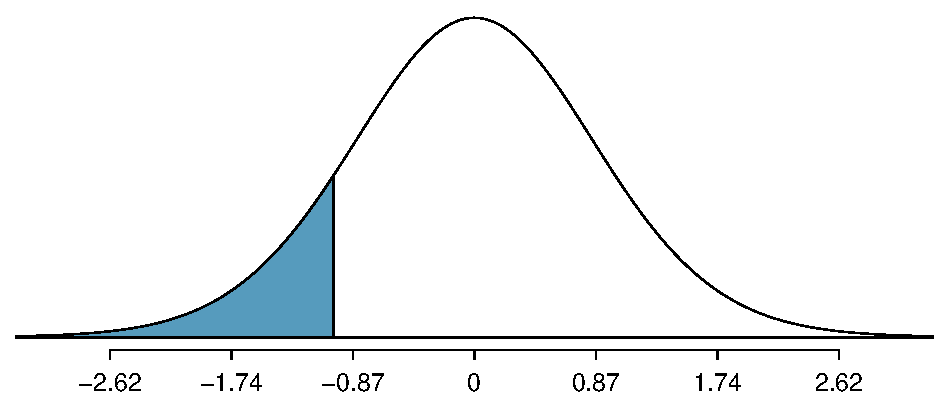
\includegraphics[width=0.82\textwidth]{ch_regr_simple_linear/figures/oneSidedTailForMidtermUnemploymentHT/oneSidedTailForMidtermUnemploymentHT}
%\caption{The distribution shown here is the sampling distribution for $b_1$, if the null hypothesis was true. The shaded tail represents the p-value for the hypothesis test evaluating whether there is convincing evidence that higher unemployment corresponds to a greater loss of House seats for the President's party during a midterm election.}
%\label{oneSidedTailForMidtermUnemploymentHT}
%\end{figure}

%\textC{\newpage}

\begin{termBox}{\tBoxTitle{Inference for regression}
We usually rely on statistical software to identify point estimates and standard errors for parameters of a regression line. After verifying conditions hold for fitting a line, we can use the methods learned in Section~\ref{oneSampleMeansWithTDistribution} for the $t$-distribution to create confidence intervals for regression parameters or to evaluate hypothesis tests.}
\end{termBox}

\begin{caution}{Don't carelessly use the p-value from regression output}{The last column in regression output often lists p-values for one particular hypothesis: a two-sided test where the null value is zero. If your test is one-sided and the point estimate is in the direction of $H_A$, then you can halve the software's p-value to get the one-tail area. If neither of these scenarios match your hypothesis test, be cautious about using the software output to obtain the p-value.}
\end{caution}


%\begin{table}[ht]
%\centering
%\begin{tabular}{rrrrr}
  %\hline
  %\vspace{-3.7mm} & & & & \\
 %& Estimate & Std. Error & t value & Pr($>$$|$t$|$) \\ 
  %\hline
  %\vspace{-3.6mm} & & & & \\
%(Intercept) & 24.3193 & 1.2915 & 18.83 & 0.0000 \\ 
%family\_\hspace{0.3mm}income & -0.0431 & 0.0108 & -3.98 & 0.0002 \\ 
  % \hline
  % \multicolumn{5}{r}{$df=48$} \\
%\end{tabular}
%\caption{A summary of least squares fit.}
%\label{rOutputForIncomeAidLSRLineInInferenceSection}
%\end{table}

\begin{tipBox}{\tipBoxTitle{Always check assumptions}
If conditions for fitting the regression line do not hold, then the methods presented here should not be applied. The standard error or distribution assumption of the point estimate -- assumed to be normal when applying the $t$-test statistic -- may not be valid.}
\end{tipBox}



Now, what does the $t(n-2)$ distribution have to do with the slope estimator $b_1$?

Well, from Equation (\ref{b1}) on page \pageref{b1}, we essentially see that $b_1$ is a linear combination of normal random variables, with the unknown variance $\sigma^2$. (The $x$-values are not random and are thus treated as constants.) Since the variance is unknown, a $t$-distribution is used in lieu of a normal distribution.


The text \emph{OpenIntro Statistics 3rd Edition} seems to neglect to clearly note that when $b_1$ is the estimated slope, under the null hypothesis that $\beta_1=0$,
we have that
\[
	T = \frac{b_1-\beta_1}{\SE(b_1)} = \frac{b_1}{\SE(b_1)}
\]
is the variable that has a $t(n-2)$ distribution. Moreover, the regression output tables provide $b_0, b_1, \SE(b_0), \SE(b_1)$ as in Table \ref{nov19}.
\begin{table}%[ht]
\centering
\begin{tabular}{rrrrr}
  \hline
  \vspace{-3.7mm} & & & & \\
 & Estimate & Std. Error & t value & Pr($>$$|$t$|$) \\ 
  \hline
  \vspace{-3.6mm} & & & & \\
(Intercept) & $b_0$ & $\SE(b_0)$ & 18.83 & 0.0000 \\ 
family\_\hspace{0.3mm}income & $b_1$ & $\SE(b_1)$ & $t$ & 0.0002 \\ 
   \hline
   \multicolumn{5}{r}{$df=48$} \\
\end{tabular}
\caption{A summary of least squares fit. The point is that ``family$\_$income'' here refers to how $y$ depends on family income. If there were more variables we would have rows for how $y$ depends on those as well: $y=\beta_0 + \beta_1x_1+\beta_2x_2+\dots$.}
\label{nov19}
\end{table}



\subsection{Statistically significant slopes when correlation coefficient is bounded away from 1}%Discussion from November 21, 2018

An important statistical distinction is that between statistical significance and \term{effect size}.
A result may be statistically significant without being ``big''.
In this section we show that the $p$-value associated with a slope can go to zero while the correlation $r^2$ is bounded away from 1.
But first, a different example.
\begin{example}{}
Imagine points $(2n,2n+1)$ and $(2n+1,2n)$. The slope $b_1$ is 1 in the limit. We have\footnote{See e.g. David E. Bock, Paul F. Velleman, and Richard D. De Veaux: \emph{Stats: Data and Models}, 4th edition.}
\[
	\SE(b_1) = \frac{\sqrt{\sum (y_i-\hat y_i)^2/(n-2)}}{\sqrt{\sum (x_i-\overline x)^2}}.
\]
(Don't forget that denominator.)
In our example, as the number of points increases, the numerator $\sqrt{\sum (y_i-\hat y_i)^2/(n-2)}$ may converge but the denominator $\sqrt{\sum (x_i-\overline x)^2}$ increases.
Thus $b_1/\SE(b_1)$ goes to $\infty$. On the other hand, $r =  b_1 s_x/s_y\approx s_x/s_y$. Now since $y\approx x$ this should all converge to 1.
\end{example}

%According to \url{https://www.andrews.edu/~calkins/math/edrm611/edrm12.htm#TESTB},
%\begin{quote}
%	Instead of testing the slope for zero ($b_1 = 0$) one can test the correlation coefficient for zero ($r = 0$). In lesson 9 we introduced the test statistic
%	\[
%		t=r\sqrt{(n-2)/(1-r^2)}.
%	\]
%	Rounding errors may slightly change the results, but that is the only difference between these two ways of checking for the significance of the regression.
%\end{quote}
%but this doesn't deal with whether $r\approx 1$.
\begin{thm}\label{frischwe}
$\sum\hat y = \sum y$.
\end{thm}
\begin{proof}
 We have
 \[
 	\frac1n\sum y = \overline y = b_0+b_1\overline x = \frac1n\left(nb_0+b_1\sum x\right) = \frac1n\sum(b_0+b_1x)=\frac1n\sum\hat y.\qedhere
\]
 \end{proof}
 
 The following Theorem \ref{ssethm} is often described as follows: the total variation is the sum of the explained variation and the residual variation.
 That is, define $\ESS$ (explained sum of squares), $\TSS$ (total sum of squares), $\RSS$) (residual sum of squares) by
 \begin{eqnarray*}
 	\ESS &=& \sum (\hat y-\overline y)^2\\
	\TSS &=& \sum(y-\overline y)^2 = (n-1)s_y^2\\
	\RSS &=& \sum(y-\hat y)^2
 \end{eqnarray*}
 The term ``sum of squares'' may seem unhelpful, until you learn that it is to be compared to \term{mean squares}, which is a sum of squares divided by its number of degrees of freedom.
 \begin{thm}[Sum of squares decomposition]\label{ssethm}
	\[
		\label{SSE}
		\TSS = \sum(y-\overline y)^2 = \sum (\hat y-\overline y)^2 + \sum(y-\hat y)^2 = \ESS + \RSS.
	\]
\end{thm}
\begin{proof}
	We need
	%\[
	%	(\hat y-\overline y)(y-\hat y) = \hat y\bullet y - \hat y\bullet \hat y  - \overline y\bullet y + \overline y\bullet \hat y
	%\]
	%not a good way:
	\begin{eqnarray*}
		\sum y^2 - 2y\overline y + \overline y^2 &=& \sum \hat y^2-2\hat y\overline y + \overline y^2 + y^2 - 2y\hat y + \hat y^2\\
		\sum  - 2y\overline y  &=& \sum 2\hat y^2-2\hat y\overline y   - 2y\hat y \\
		-2n\overline y^2  &=& \sum 2\hat y^2- \sum 2\hat y\overline y   - \sum 2y\hat y \\
		-\sum y\overline y  &=& \sum \hat y^2- \sum \hat y\overline y   - \sum y\hat y \\
		 \sum \hat y\overline y   + \sum y\hat y &=& \sum y\overline y   +  \sum \hat y^2
	\end{eqnarray*}
	Now by Theorem \ref{frischwe}, $\sum\hat y = \sum y$, so we just need
	\begin{eqnarray*}
		  \sum y\hat y &=&   \sum \hat y^2\\
		  \sum y(b_0+b_1x) &=&   \sum (b_0+b_1x)^2\\
		  b_0\overline y + b_1 \overline {xy} &=& b_0^2 + 2b_0b_1\overline x + b_1^2\overline{x^2}\\
		  (\overline y-b_1\overline x)\overline y + b_1 \overline {xy} &=& (\overline y-b_1\overline x)^2 + 2(\overline y-b_1\overline x)b_1\overline x +b_1^2 \overline{x^2}\\
		  b_1 \overline {xy} &=& (\overline y-b_1\overline x)(-b_1\overline x) + 2(\overline y-b_1\overline x)b_1\overline x + b_1^2\overline{x^2}\\
		  b_1 \overline {xy} &=& (\overline y-b_1\overline x)b_1\overline x +b_1^2 \overline{x^2}\\
		b_1(\overline{xy} - \overline x\cdot\overline y) &=& b_1^2\overline{x^2} - b_1^2\overline{x}^2
	\end{eqnarray*}
	which upon dividing by $b_1$ is our formula for $b_1$ from Equation (\ref{b1}).
\end{proof}

\begin{thm}\label{aid}
$1-r^2= \frac{\sum(y-\hat y)^2/(n-1)}{s_y^2}$.
\end{thm}
\begin{proof}
	\begin{eqnarray*}
		1-r^2 												&\overset{!}{=}& \frac{\sum(y-\hat y)^2/(n-1)}{s_y^2}\\
		1-(b_1s_x/s_y)^2 										&\overset{!}{=}& \frac{\sum(y-\hat y)^2/(n-1)}{s_y^2}\\
		s_y^2-(b_1s_x)^2 										&\overset{!}{=}& \frac{\sum(y-\hat y)^2}{n-1}\\
		\sum(y-\overline y)^2-b_1^2 \sum (x-\overline x)^2 				&\overset{!}{=}& \sum(y-\hat y)^2\\
		\sum(y-\overline y)^2 - \sum (b_0+b_1x-(b_0+b_1\overline x))^2 	&\overset{!}{=}& \sum(y-\hat y)^2\\
		\sum(y-\overline y)^2 - \sum (\hat y-\overline y)^2 				&\overset{!}{=}& \sum(y-\hat y)^2\\
		\sum(y-\overline y)^2										&\overset{!}{=}& \sum (\hat y-\overline y)^2 + \sum(y-\hat y)^2
	\end{eqnarray*}
	which is true by Theorem \ref{ssethm}.
	%good way: we claim the vectors $\hat y-\overline y$ and $y-\hat y$ are orthogonal.
\end{proof}

\begin{thm}\label{miao-hu}
\[
r^2=\frac{\ESS}{\TSS}=\frac{\sum (\hat y-\bar y)^2}{\sum (y-\bar y)^2}.
\]
\end{thm}
\begin{proof}
We have
\[
	1-r^2= \frac{\sum(y-\hat y)^2/(n-1)}{s_y^2} = \frac{[\sum(y-\bar y)^2-\sum (\hat y-\bar y)^2]/(n-1)}{s_y^2} = 1-\frac{\sum (\hat y-\bar y)^2/(n-1)}{s_y^2}.
\]
\end{proof}
 
\begin{thm}\label{https://www.andrews.edu/}
The $t$ statistic $t=b_1/\SE(b_1)$ is also given by
	\[
		t=r\sqrt{(n-2)/(1-r^2)}.
	\]
\end{thm}

Note that $r/\sqrt{1-r^2}$ goes to $\infty$ only when $r\to 1$, but $\sqrt{n-2}$ goes to infinity anyway. So if $r$ is a fixed value (there is a certain amount of spread around the regression line and it's not going away) then we should achieve statistical significance as $n\to \infty$. Namely, imagine that $X$ and $Y$ are correlated jointly normal random variables with a correlation coefficient $\rho$; for large $n$ we will have $r\approx\rho$.
\begin{proof}[Proof of Theorem \ref{https://www.andrews.edu/}]
	\begin{eqnarray*}
		\frac{b_1}{\SE(b_1)}										&\overset{!}{=}& \frac{r\sqrt{n-2}}{\sqrt{1-r^2}}\\
		\frac{r s_y}{s_x \SE(b_1)} 									&\overset{!}{=}& \frac{r\sqrt{n-2}}{\sqrt{1-r^2}}\\
		\frac{s_y}{s_x \SE(b_1)}									&\overset{!}{=}& \frac{\sqrt{n-2}}{\sqrt{1-r^2}}\\
		\frac{s_y^2}{s_x^2 \SE(b_1)^2}								&\overset{!}{=}& \frac{n-2}{1-r^2}\\
		\frac{s_y^2}{s_x^2 \frac{\sum(y-\hat y)^2/(n-2)}{(n-1)s_x^2}}		&\overset{!}{=}& \frac{n-2}{1-r^2}\\
		\frac{s_y^2}{\frac{\sum(y-\hat y)^2/(n-2)}{(n-1)}}					&\overset{!}{=}& \frac{n-2}{1-r^2}\\
		\frac{s_y^2}{\sum(y-\hat y)^2/(n-1)} 							&\overset{!}{=}& \frac{1}{1-r^2}\\
		1-r^2 												&\overset{!}{=}& \frac{\sum(y-\hat y)^2/(n-1)}{s_y^2}\\
	\end{eqnarray*}
which is true by Theorem \ref{aid}.
\end{proof}


Consequently, we can also express $r^2$ in terms of $t$;
\begin{eqnarray}
	t&=&r\sqrt{(n-2)/(1-r^2)}\\
\label{goat}	t^2&=&r^2(n-2)/(1-r^2)\\
	(1-r^2)t^2&=&r^2(n-2)\\
	t^2&=&r^2(n-2+t^2)\\
	r^2 &=& \frac{t^2}{t^2+n-2}
\end{eqnarray}
It is also instructive to express $t^2$ by
\begin{equation}\label{hu}
	t^2 = \frac{r^2(n-2)}{1-r^2} = \frac{(n-2)\ESS/\TSS}{1-\ESS/\TSS}=\frac{(n-2)\ESS}{\TSS-\ESS}%=\frac{(n-2)\ESS}{\RSS}
	= \frac{\ESS/1}{\RSS/(n-2)}
\end{equation}
Without explaining it in detail, we remark that in the equation
\[
	\underbrace{\TSS}_{n-1 \text{ df}} = \underbrace{\ESS}_{1 \text{ df}} + \underbrace{\RSS}_{n-2 \text{ df}}
\]
we have $n-1$ df for $\TSS$, which breaks down into $1$ df for $\ESS$ and $n-2$ df for $\RSS$.
The ratio in (\ref{hu}) has an \term{$F$ distribution} $F(df_1,df_2)$ where $df_1=1$ and $df_2=n-2$.
Thus if we define a random variable $F=t^2$, we have for in the simple linear regression setting that
\[
r^2 = \frac{F}{F+df_2/df_1}.
\]

There is an underlying algebraic lemma here:
\begin{lem}
Let $F$, $a$, $u_1$, $u_2$, $r$ be numbers.
If $F=\frac{a/u_1}{b/u_2}$ and $r^2=\frac{a}{a+b}$, then $F$ and $r^2$ are related by
\[
	r^2 = \frac{F}{F+u_2/u_1}.
\]
\end{lem}
\begin{proof}
We calculate:
\[
	\frac{F}{F+u_2/u_1} = \frac{\frac{a/u_1}{b/u_2}}{\frac{a/u_1}{b/u_2} + u_2/u_1} = \frac{a/u_1}{a/u_1+b/u_1}=r^2.\qedhere
\]
\end{proof}
%It seems from https://msu.edu/~levinet/eta%20squared%20hcr.pdf that partial eta squared, rather than eta squared, is associated with the lemma above.


We cannot recover $a$ and $b$ from $F$, $r^2$, $u_1$ and $u_2$, but we can recover their ratio $a/b$.
%\[
%	F=\frac{a/u_1}{b/u_2},\quad r^2=\frac{a}{a+b}
%\]
%\[
%	Fb/u_2=a/u_1,\quad (a+b)r^2=a
%\]
%\[
%	Fbu_1=au_2,\quad b = a(1-r^2)/r^2
%\]
%\[
%	F[a(1-r^2)/r^2]u_1=au_2
%\]
%\[
%	a/b=r^2/(1-r^2)
%\]
%\[
%	F[(1-r^2)/r^2]u_1=u_2
%\]


	%Well the whole point was to minimize $\sum (y-\hat y)^2=\sum y^2-2y\hat y + \hat y^2$
	%i.e., to set $\partial \sum \hat y^2-2y\hat y=0$.
	%\[
	%	\sum 2\hat y \partial \hat y - 2y \partial\hat y =0
	%\]



\subsection{Multiple regression}
In the multiple regression case $k>1$
this generalizes to an $F(n-k-1, k)$ distribution\footnote{See \texttt{https://www3.nd.edu/\~rwilliam/stats2/l02.pdf}} for 
\[
	F
	= \RMS/\EMS
	= \frac{\RSS/(n-k-1)}{\ESS/(k)}
	= \frac{r^2(n-k-1)}{(1-r^2)k}
\]
but RSS and ESS are calculated the same, as they are not really about the $x$'s.
%We can investigate how this works for a fixed data set like the ``maximum function'':
%\[
%	(0, 0, 0),
%	(0, 1, 1),
%	(1, 0, 1),
%	(1, 1, 1)
%\]

The standard error associated with a slope $b_1$ for a model $z=a+bx+cy$ is\footnote{See \texttt{nd.edu/\~rwilliam/stats1/x91.pdf}}
\[
	\SE(b_1) = \frac{s_z}{s_x} \sqrt{\frac{1-r^2_{z,(x,y)}}{(1-r^2_{x,y})(n-k-1)}}
\]
where $k=2$ for the two explanatory variables $x,y$.
Let us investigate how regression works for the model $z=a+bx+cy$ or equivalently $z=a+b_1x+b_2y$.

We seek $a,b,c$ to minimize $f(a,b,c)=\sum (z_i-a-bx_i-cy_i)^2$.
Setting the partial derivatives equal to zero we get
\begin{eqnarray*}
\begin{pmatrix} \overline z \\ \overline{xz} \\ \overline{yz}\end{pmatrix} = \begin{pmatrix}
	1 & \overline x & \overline y \\
	\overline x & \overline{x^2} & \overline{xy} \\
	\overline y & \overline{xy} & \overline{y^2}
\end{pmatrix}
\begin{pmatrix}
a \\ b\\ c
\end{pmatrix}
\end{eqnarray*}
With some matrix algebra this gives, besides $a=\overline z-b\overline x-c\overline y$, and in terms of the shorthands $\cov(x,y)=\overline{xy}-\bar x\bar y$ and $\vari(x)=\cov(x,x)$, that
\[
	\slope^{(2)}_{z,x} := b = \frac{\cov(x,z)\vari(y)-\cov(y,z)\cov(x,y)}{\vari(x)\vari(y)-(\cov(x,y))^2}
\]
To understand this we introduce the notation $\slope^{(1)}_{y,x} = \frac{\cov(x,y)}{\vari(x)}$ which happens to be the slope for the simpler model $y=a+bx$.
Then we can write
\[
	b = \frac{\slope^{(1)}_{z,x} - \slope^{(1)}_{z,y} \slope^{(1)}_{y,x}}{1-r^2_{x,y}}
\]
since $r_{xy}^2=\frac{\cov(x,y)^2}{\vari(x)\vari(y)}$. (We sometimes write a subscript $x,y$ as simply $xy$.)

Now in the formula for SE($b_1$) above, the term $r_{z,(x,y)}$ represents the correlation between $z$ and the best-fitting approximation to $z$ by any linear combination of $x$ and $y$. It is given\footnote{
	See \texttt{https://en.wikipedia.org/wiki/Multiple\_correlation}.
} by
\begin{eqnarray*}
	r^2_{z,(x,y)} &=& \begin{pmatrix} r_{x,z} & r_{y,z}\end{pmatrix} \begin{pmatrix} r_{xx}& r_{xy} \\ r_{xy} & r_{yy} \end{pmatrix}^{-1} \begin{pmatrix} r_{xz}\\ r_{yz}\end{pmatrix}\\
	&=&\frac{r_{xz}^2+r_{yz}^2-2r_{xy}r_{yz}r_{zx}}{1-r_{xy}^2}
\end{eqnarray*}
where we have done some matrix algebra in the last step.
Now let us consider
\[
	F_1 = t_1^2 = b_1^2/\SE(b_1)^2
\]
and similarly $F_2$.

Now\footnote{See \texttt{http://www.stat.yale.edu/Courses/1997-98/101/anovareg.htm}} the appropriate $F$-statistic for testing whether $\beta_1=\beta_2=0$ (where $\beta$ is the ``true'' parameter being estimated by $b$) is
\[
	F
	%= \frac{mean square model}{mean square error}
	=\frac{\EMS}{\RMS}
	%= \frac{sum of squares model / df model}{sum of squares error / df error}
	=\frac{\ESS/d_1}{\RSS/d_2}
	=\frac{\sum (\hat z-\overline z)^2/p}{\sum(z-\hat z)^2/(n-p-1)}
\]
where $p=2$ is the number of explanatory variables. This has an $F(p,n-p-1)$ distribution.
Doing the algebra we see that the numerator of $F$ is 
\[
	\vari(x) (\SE(b_1))^2 \left[ t_1^2+t_2^2 + 2t_1t_2 \frac{\cov(x,y)}{\vari(y)}\right].
\]
Thus the two $F$ statistics $F_1$ and $F_2$ are combined nontrivially to form $F$, except if we ensure that $\cov(x,y)=0$.
We may note that $\SE(b_1)=\SE(b_2) s_y/s_x$ and $\slope^{(1)}_{xy}\slope^{(1)}_{yx}=r_{xy}^2$.
Also $F_1$ gets the interesting form
\[
	(n-p-1)\frac{r_{zx}^2+r_{zy}^2r_{yx}^2 - 2r_{xy}r_{yz}r_{zx}}{1-r_{xy}^2-r_{yz}^2-r_{xz}^2+2r_{xy}r_{yz}r_{xz}}
	=
	(n-p-1)\frac{(r_{zx}-r_{zy}r_{yx})^2}{1-r_{xy}^2-r_{yz}^2-r_{xz}^2+2r_{xy}r_{yz}r_{xz}}.
\]
\[
	=
	(n-p-1)\frac{(r_{zx}-r_{zy}r_{yx})^2}{1- (r_{xz}-r_{xy}r_{yz})^2+r_{xy}^2r_{yz}^2-r_{xy}^2-r_{yz}^2}.
\]
which mimics (\ref{goat}) if we take the $y$ terms to be 0, $r_{xy}=r_{yz}=0$.

We have
\[
	\frac{F}{F+(n-p-1)/p} = \frac{\ESS}{\RSS+\ESS}.\tag{*}
\]

Let us write $\ESS_x$ for the explained sum of squares in the case where we only use $x$ (and not $y$) in our model.
If we have independent variables $x$, $y$, then values of the effect size measure
\[
\eta^2(x):=\frac{\ESS_x}{\RSS+\ESS}
\]
can be added\footnote{See \texttt{https://msu.edu/~levinet/eta\%20squared\%20hcr.pdf}.},
\[
\eta^2(x)+\eta^2(y)=\frac{\ESS_x}{\RSS+\ESS} + \frac{\ESS_y}{\RSS+\ESS}\le 1
\]
%Levine and Hullett, Eta squared ...

as $x$ and $y$ cannot explain the same variation (see Subsection \ref{levine-hullett-claim}). But with partial $\eta^2$, 
\[
\eta^2_p(x):=\frac{\ESS_x}{\RSS+\ESS_x}
\]
a sum like
\[
\eta_p^2(x)+\eta_p^2(y)=\frac{\ESS_x}{\RSS+\ESS_x} + \frac{\ESS_y}{\RSS+\ESS_y}
\]
gives no such control. It is the partial form that satisfies (*) given that $F=\EMS_x/\RSS$.
If we want to completely throw out the independent variables other than $x$ we could replace $\RSS$ by $\RSS_x$.

%the t statistic from paired tests fits into this?
\subsection{Adding the variation explained by $x$ and $y$}\label{levine-hullett-claim}

If $x$ and $y$ are independent in some sense then they explain different parts of the sum of squares.
\begin{example}{Perfect fit.}
If actually $z=x+y$ is a perfect fit and $(0,0), (0,1), (1,0), (1,1)$ are the values for $(x,y)$, then $\bar z = 1$ and $\TSS = (0-1)^2+(2-1)^2 = 2$
but if we only consider $x$ then we see $0$ maps to $1/2$ and $1$ maps to $3/2$ so maybe $z=x+1/2$ is the best fit.
The ESS for $x$ is then $2 (1/2-1)^2 + 2(3/2-1)^2 = 1$ and similarly for $y$.
\end{example}

This is reminiscent of the fact that if $X$ and $Y$ are independent random variables (or more generally just uncorrelated) then $\Var(aX+bY)=\Var(aX)+\Var(bY)$. In ``found data'' independence usually does not obtain, but in a controlled experiment it usually does.


The variation explained by $x$ is
\[
	\ESS_x = \sum (\overline z - \slope^{(1)}_{z,x}x-\intercept_{z,x})^2
\]
Here $\intercept_{z,x}$ is defined by
\[
	\overline z = \slope^{(1)}_{z,x}\overline x + \intercept_{z,x}
\]
so
\[
	\ESS_x = \sum (\overline z - \slope^{(1)}_{z,x}x- [\overline z - \slope^{(1)}_{z,x}\overline x]  )^2
\]
\[
	= \sum ( - \slope^{(1)}_{z,x}x- [ - \slope^{(1)}_{z,x}\overline x]  )^2 = (\slope^{(1)}_{z,x})^2 \vari(x)\cdot n = \cov(z,x)^2n/\vari(x).
\]
Similarly $\ESS_y = \cov(z,y)^2n/\vari(y)$.
So
\[
\ESS_x+\ESS_y = \frac{\cov(z,x)^2n}{\vari(x)} + \frac{\cov(z,y)^2n}{\vari(y)} = n \frac{(\cov(z,x)^2\vari(y)+\cov(z,y)^2\vari(x)}{\vari(x)\vari(y)}
\]
On the other hand,
\[
	\ESS = \sum (\overline z - bx-cy -\intercept_{z,(x,y)})^2
\]
where $\intercept_{z,(x,y)}=\overline z - b\overline x-c\overline y$, so
\[
	\ESS = \sum (\overline z - bx-cy -[\overline z - b\overline x-c\overline y])^2 = \sum (- bx-cy -[ - b\overline x-c\overline y])^2
\]
\[
	= \sum (b(x-\overline x)+c(y-\overline y))^2 = b^2 n\vari(x) + c^2n\vari(y) + 2bcn\cov(x,y)
\]
This does not immediately have the result
\begin{equation}\label{resu}
\cov(x,y)=0 \implies \ESS=\ESS_x+\ESS_y
\end{equation}
as there is a difference between $b=\slope^{(2)}_{z,x}$ and $\slope^{(1)}_{z,x}$:
\[
	b = \frac{\slope^{(1)}_{z,x} - \slope^{(1)}_{z,y} \slope^{(1)}_{y,x}}{1-r^2_{x,y}}
\]
However, if $\cov(x,y)=0$ then $r_{x,y}=0$ and also $\slope^{(1)}_{y,x}=0$. So we do get (\ref{resu}).

\begin{example}{Necessity of covariance zero.}
It is possible to have $\cov(x,y)<0$ and $b,c>0$, leading to $\ESS_x+\ESS_y>\ESS$. Just consider the example
\[
	\{(1,0),(1,1),(0,1)\}
\]
with $z=x+y$ again.
\end{example}

\section{ANOVA}
We perform an Analysis of Variance (ANOVA) with three groups (i.e., $p=3$). Group A consists of students who turned in Assessment Exam III on time, and reported that they had taken MATH 412 (Introduction to Abstract Algebra). Following the notation of \footfullcite[Section 11.6]{degroot2011probability}, the scores on the Pilot Assessment Exam in Group A were
\[
	(Y_{1,1},Y_{1,2}) = (5, 13)
\]
with a group mean of
\[
	\overline Y_{1+} = 9.
\]
Group B consists of students who turned in Assessment Exam III on time, and reported that they had \emph{not} taken MATH 412.
The scores on the Pilot Assessment Exam in Group B were
\[
	(Y_{2,1},Y_{2,2}) = (6, 8)
\]
with a group mean of
\[
	\overline Y_{2+} = 7.
\]
Group C consists of students who did not turn in Assessment Exam III on time.
The scores on the Pilot Assessment Exam in Group C were
\[
	(Y_{3,1},\dots,Y_{3,6}) = (2, 3, 6, 7, 8, 10)
\]
with a group mean of
\[
	\overline Y_{3+} = 6.
\]
Let $(n_1,n_2,n_3)=(2,2,6)$ and $n=\sum_{i=1}^p n_i=10$.
The grand mean is
\[
	\overline Y_{++} = \frac{2\overline Y_{1+}+2\overline Y_{2+}+6\overline Y_{3+}}{10} = \frac{18+14+36}{10} = 6.8.
\]
The residual sum of squares is
\[
	SS_{\text{within}} = \sum_{i=1}^p \sum_{j=1}^{n_i}(Y_{i,j}-Y_{i+})^2 = (5-9)^2+(13-9)^2\quad +\quad (6-7)^2+(8-7)^2
\]
\[
	+ (2-6)^2+(3-6)^2+(6-6)^2+(7-6)^2+(8-6)^2+(10-6)^2
\]
\[
	= 16+16+1+1+16+9+0+1+4+16 = 64+9+4+3+0 = 80.
\]
The ``between-sample-means'' or ``factor'' sum of squares is
\[
	SS_{\text{between}} = \sum_{i=1}^p n_i(\overline Y_{i+}-\overline Y_{++})^2
\]
\[
	= 2(9-6.8)^2 + 2(7-6.8)^2 + 6(6-6.8)^2 = 2(2.2)^2+2(0.2)^2+6(0.8)^2 = 13.6.
\]
The test statistic is
\[
	U^2 = \frac{SS_{\text{between}}/(p-1)}{SS_{\text{within}}/(n-p)} = \frac{13.6/(3-1)}{80/(10-3)} = \frac{6.8}{11.42857} = 0.595.
\]
When compared to an $F(p-1,n-p)=F(2,7)$ distribution, we would need a value of 4.74 to reject the null hypothesis that the means are equal at the $95\%$ level.
While the data are consistent with the idea that punctuality, and taking MATH 412, both lead to better scores, we cannot reject the null hypothesis that these things have no effect.

\subsection{$2\times 2$ ANOVA}
Interaction between two variables that together produce an effect is studied in $2\times 2$ ANOVA\footnote{Source: \texttt{https://www4.uwsp.edu/psych/stat/13/anova-2w.htm}}.

The idea of interaction between factors can be illustrated in several examples.
\begin{example}{Sandwich ingredients.}
Suppose you make a sandwich using bread and some of the four ingredients peanut butter, herring, tomato, and avocado. Which combinations would yield a tasty sandwich? Perhaps each ingredient is tasty by itself, but some combinations are not.
\end{example}

\begin{example}{Addition mod 2.}
Suppose you consider $X+Y+Z$ mod 2. No information about one or two of the variables gives you any information; you need all three, at which point you have complete information.
\end{example}

\begin{example}{Black cats crossing the street in front of you.}
Suppose you are superstitious and worry if you see a black cat crossing the street in front of you. However, you need all the four aspects for the superstition to apply. Thus, a black cat crossing the street all alone is not a problem, neither is a black cat in front of you a problem if it's not crossing the street, and so on.
\end{example}


Since the GRE data has a missing group, let's apply the theory instead to presidents: Democrat or Republican, 2-term or 1-term, and look at their height.
Let's take the last 3 of each.

\begin{table}
	\begin{tabular}{|c|c|c|}
		\hline
		& 1-term & 2-term \\
		\hline
		D & Carter 5'10'', JFK 6'0'', Cleveland 5'11'& Obama 6'1'', Clinton 6'2'', LBJ 6'4'' \\
		R & GHW Bush 6'2'', Ford 6'0'', Hoover 6'0''& GW Bush 6'0'', Reagan 6'2'', Nixon 5'11'' \\
		\hline
	\end{tabular}
\begin{minipage}{0.5\textwidth}
	\begin{tabular}{|c|c|c|}
		\hline
		Inches above 5'10''& 1-term & 2-term \\
		\hline
		Democrat & 0,1,2& 3,4,6 \\
		Republican & 2,2,4& 1,2,4 \\
		\hline
	\end{tabular}
\end{minipage}
\begin{minipage}{0.5\textwidth}
	\begin{tabular}{|c|c|c|c|}
		\hline
		Means& 1-term & 2-term &\\
		\hline
		D & 1.00      & 4.33 & 2.667\\
		R & 2.67   & 2.33 & 2.500\\
		\hline
		 & 1.833   & 3.333  & 2.583\\
		\hline
	\end{tabular}
\end{minipage}
\caption{Height of U.S.~Presidents by party and number of terms.}\label{pres}
\end{table}
%\begin{itemize}
%\item 1-term Democrat (Carter 5'10'', JFK 6'0'', Cleveland 5'11')
%\item 2-term Democrat (Obama 6'1'', Clinton 6'2'', LBJ 6'4'')
%\item 1-term Republican (GHW Bush 6'2'', Ford 6'0'', Hoover 6'0'')
%\item 2-term Republican (GW Bush 6'0'', Reagan 6'2'', Nixon 5'11'')
%\end{itemize}
Since 5'10'' is the shortest, let's look at the number of inches above that (Table \ref{pres}).


At first glance it seems that D vs.~R makes very little difference, but 2-term presidents are taller than 1-term presidents. 
Really, though, most striking is that Democratic 2-term presidents are very tall, Democratic 1-term presidents very short, and Republicans somewhere in the middle regardless of number of terms.

With $n=3$ and $p=q=2$ being the number of levels of the factors, and with D vs.~R being ``factor A'', we can write
\[
	X_{111},X_{211},X_{311}=0,1,2,\quad X_{121},X_{221},X_{321}=2,2,4
\]
\[
	X_{112},X_{212},X_{312}=3,4,6,\quad X_{122},X_{222},X_{322}=1,2,4
\]
(thus the convention for index order is backwards from the GRE example above)
\[
	\overline X_{11}=\frac{0+1+2}3=1,\quad \overline X_{12}=\frac{2+2+4}3=2.67,\quad\overline X_{21}=\frac{3+4+6}3=4.33,\quad \overline X_{22}=3.33
\]
\[
	\overline X_{1\cdot} = 2.667,\quad \overline X_{2\cdot}=2.500,\quad \overline X_{\cdot 1}=1.833,\quad \overline X_{\cdot 2}=3.333,\quad \overline X_{\cdot\cdot} = 2.583
\]
Now we have five sums of squares, $SS_T$ (total), $SS_A$ (effect of factor $A$), $SS_B$, $SS_{A\times B}$ (interaction of $A$ and $B$), $SS_{\text{within}}$ (error, unexplained variance, within cells).
\begin{eqnarray*}
	SS_A			&=& nq \sum_{j=1}^p (\overline X_{j\cdot}-\overline X_{\cdot\cdot})^2\\
	SS_B			&=& np \sum_{k=1}^q (\overline X_{\cdot k}-\overline X_{\cdot\cdot})^2\\
	SS_{A\times B} 	&=& n \sum_{j=1}^p\sum_{k=1}^q ([\overline X_{jk}-\overline X_{\cdot\cdot}] - [\overline X_{j\cdot}-\overline X_{\cdot\cdot}] - [\overline X_{\cdot k}-\overline X_{\cdot\cdot}] )^2\\
	SS_{\text{within}} 	&=& \sum_{i=1}^n \sum_{j=1}^p\sum_{k=1}^q (X_{ijk}-\overline X_{jk})^2\\
	SS_T			&=& \sum_{i=1}^n \sum_{j=1}^p\sum_{k=1}^q (X_{ijk}-\overline X_{\cdot\cdot})^2\\
\end{eqnarray*}
The degrees of freedom are as follows.
\begin{eqnarray*}
	df_A				&=& p-1=1\\
	df_B				&=& q-1=1\\
	df_{A\times B}		&=& (p-1)(q-1)=pq-p-q+1=1\\
	df_{\text{within}}	&=& pq(n-1)=pqn-pq=N-pq\\
	df_T				&=& npq-1=N-1
\end{eqnarray*}
Note that
\[
	df_T = df_A + df_B + df_{A\times B} + df_{\text{within}}
\]
It can also be shown that
\[
	SS_T = SS_A + SS_B + SS_{A\times B} + SS_{\text{within}}
\]
For our $F$ tests we take the relevant mean squares in the numerator and mean squares for error $MS_{\text{within}}$ in the denominator as usual. As they nicely put it,
\[
	MS=SS/df\quad \text{and} \quad F=MS_{\text{source}}/MS_{\text{error}}.
\]
Note the difference between saying there is an $A\times B$ effect (the interaction between $A$ and $B$ is significant, e.g., Democratic presidents are taller the more terms they serve) and saying that $x$ and $y$ are correlated in the regression section above (there, we could just set $x$ and $y$ to be independent by design, and we were only interested in predicting $z$ from $x$ and $y$, not in discovering that $x$ and $y$ were correlated or interacting).

In our example we get $SS_A=\frac1{12}$, $SS_B=\frac{27}4$, $SS_{\text{within}}=14$, $SS_{A\times B}=10+\frac1{12}$. While computing $SS_{A\times B}$ by hand we notice that for a $2\times 2$ ANOVA like this the formula simplifies to
\[
	SS_{A\times B} = npq (\overline X_{jk}-\overline X_{\cdot\cdot})^2
\]
for any particular $1\le ,j, k,\le 2$, i.e., the quantity does not depend on $j$ and $k$. This is an expression of the fact that $df_{A\times B}=1$.
To test for $A\times B$ interaction, we compute
\[
	F = \frac{SS_{A\times B}/df_{A\times B}}{SS_{\text{within}}/df_{\text{within}}} = \frac{(10+\frac1{12})/1}{14/8} = 5+\frac{16}{21} = 5.7619.
\]
and $F(1,8)=5.7619$ gives a $p$-value of $.04315$. Thus, the interaction between political party and number of terms for a U.S.~President is significant for height at the usual 5\% level.

\paragraph{An example from marketing research.}
The data in Table \ref{RuckerHuGalinsky} is taken from \footfullcite[pages 386--387]{doi:10.1086/676598}.
\begin{table}
\centering
\begin{tabular}{|c|c|c|c|}
\hline
focus$\backslash$ power	&	low	& high & marginal of focus\\
\hline
experience			& 	2.17 & 1.16 & =1.665\\
expectations			&	1.39 & 2.31 & =1.850\\
\hline
marginal of power		&	1.780 & 1.735 & = 1.7575\\
\hline
\end{tabular}
\begin{tabular}{|c|c|c|}
\hline
focus$\backslash$ power	&	low	& high \\
\hline
experience			& 	1.78 & 1.82 \\
expectations			&	1.62 & 1.56 \\
\hline
\end{tabular}
\caption{Means and standard deviations of willingness to buy, on a Likert scale.}\label{RuckerHuGalinsky}
\end{table}

It seems clear, or plausible, that the marginals are not significant.

For the power $\times$ focus interaction they report $F(1,144)=12.84, p<0.01, \eta_p^2=0.08$. This fits with our relationship between $F$, df, and $\eta_p^2$ above.
\begin{itemize}
\item For the ``experience'' row they report $F(1,144)=6.88, p=.01, \eta_p^2=0.07$.
We find
\[
	F:= t^2= \left((2.17-1.16)/\sqrt{1.78^2/37+1.82^2/37}\right)^2=2.4^2=5.82.
\]
The degrees of freedom should be $2n-2=2(n-1)=72$ which fits their reported $\eta_p^2$:
if $F(1,72)=5.82$ then $\eta^2_p=F/(F+72)=5.82/(5.82+72)=0.07$.
They state that they are using a between-subject design (p.~385) which suggests there may be $148/4=36$ individuals per group.
\item For the ``expectations'' row they report $F(1,144)=5.03, p=.03, \eta_p^2=0.08$.
We find
\[
	F:=t^2=\left((1.39-2.31)/\sqrt{1.62^2/37+1.56^2/37}\right)^2=6.20.
\]
The degrees of freedom should be $2n-2=2(n-1)=72$ which fits their reported $\eta_p^2$:
%if $F(1,144)=6.2$ then $\eta^2_p=F/(F+144)=6.2/(6.2+144)=0.04$ but
if $F(1,72)=6.2$ then $\eta^2_p=F/(F+72)=6.2/(6.2+72)=0.08$.
%and if $F(1,72)=5.03$ then $\eta^2_p=F/(F+72)=5.03/(5.03+72)=0.065$. %But maybe the point is that the same participants tried different focuses.
\end{itemize}
%These $\eta_p^2$ values do not fit our relationship between $F$, df, and $\eta_p^2$ above.
%So the question now is how to test individual interactions like this.
We have
\[
SS_{A\times B}/n=	4   [(2.17-1.7575)-(1.665-1.7575)-(1.780-1.7575)]^2\\
	%&+& [(1.16-1.7575)-(1.665-1.7575)-(1.735-1.7575)]^2\\
	%&+& [(1.39-1.7575)-(1.850-1.7575)-(1.780-1.7575)]^2\\
	%&+& [(2.31-1.7575)-(1.850-1.7575)-(1.735-1.7575)]^2\\
	=0.931225
\]
and hence $SS_{A\times B} = 34.455325$.
In this case $df_{\text{within}}=144=N-pq$ where $N=148$, $p=2$, $q=2$, and presumably $n=N/pq=148/4=37$.

$SS_{\text{within}}$ can be figured out from the standard deviations given in Table \ref{RuckerHuGalinsky}.
So
\[
	SS_{\text{within}}=(37-1)(1.78^2+1.82^2+1.62^2+1.56^2)=415.3968
\]
should be the sum of all deviations between individual observations and their respective group means.
The $F$ statistic should then be
\[
F=\frac{MS_{A\times B}}{MS_{\text{within}}}=\frac{SS_{A\times B}/df_{A\times B}}{SS_{\text{within}}/df_{\text{within}}}=\frac{34.45/1}{415.3968/144}=11.94.
\]
which is fairly close to the stated 12.84.
%Incidentally the $SS_{A\times B}/n$ breaks down by row as:
%\begin{eqnarray*}
%SS_{A\times B}/n (row 1)&=&	   [(2.17-1.7575)-(1.665-1.7575)-(1.780-1.7575)]^2\\
%	&+& [(1.16-1.7575)-(1.665-1.7575)-(1.735-1.7575)]^2=0.4656125\\
%SS_{A\times B}/n (row 2)&=&\\
%	&+& [(1.39-1.7575)-(1.850-1.7575)-(1.780-1.7575)]^2\\
%	&+& [(2.31-1.7575)-(1.850-1.7575)-(1.735-1.7575)]^2=0.4656125\\
%\end{eqnarray*}

\subsection{Permutation tests}%Thanks to Barb and Cherryle
Permutation tests were introduced in Section 6.2.2 of \emph{OpenIntro Statistics} in the context of a difference of means.

Consider our example of the heights of U.S.~Presidents. Is the mean height for Democrats large?
Taking all the heights and considering all the permutations of them, there may seem to be $12!$ choices to consider. Doing so, we find that 
\[
	179365520/(179365520+299634480) = 37\%
\]
of the permutations give a larger mean. Thus we have a $p$-value of .37 for our alternative hypothesis that Democrats are taller. Not statistically significant.

Did we really have to consider all $12!$ permutations? Clearly not, since in this case all that matters is which of the $12\choose 6$ sets of 6 Presidents was chosen. Searching through all such sets instead, we find that 578 have a smaller mean height, and 346 a larger mean height, for a total of $924={12\choose 6}$.
The $p$-value is $346/924 = 37\%$, i.e., unchanged, but our computation much faster.



We can try to permutation tests also for more complicated test statistics such as $SS_{A\times B}/SS_{\text{between}}$ above. We can ignore the degrees of freedom since they will be the same for all the permutations, and we are not claiming to be able to compare with any limiting distribution anymore. Then what we do is look at all $12!=479,001,600$ permutations of the 12 heights of U.S.~presidents, and calculate the statistics for them (or, to save time, take a random sample). The percentile that our value finds itself (in this case a computer calculation showed it to be $4.1\%$) then becomes the $p$-value.

Permutation tests are in a way more satisfying than traditional $t$- and $z$-tests. They were introduced by Fisher about 100 years ago, but were impractical before the advent of computers. They remove the need to argue for approximate normality.

On the other hand, we still have to argue that our test statistic like $SS_{A\times B}/SS_{\text{within}}$ measures what we want it to measure. If we get a low $p$-value, we can argue that the labels ``Democrat'', ``1-term'' and so on were not assigned to the heights uniformly at random.

The fact that this is evident in the $SS_{A\times B}/SS_{\text{within}}$ statistic suggests that we can also rule out that they were assigned randomly and independently with given marginal distributions. In other words, there is an interaction of being Democrat and being 1-term on the variable \emph{height}. %Perhaps, however, we should only iterate over permutations with the given row and column averages. But that may be too strict as there may not be many permutations with exactly the same marginals. For binary variables (as in Fisher's lady tasting tea experiment) this is not an issue.
To define interaction we first need conditional expectation.
The conditional expectation of a random variable $X$ given an event $A$ is just
\[
	\sum_x x \P(X=x\mid A).
\]
Now, the definition of $P$ and $Q$ having no \term{interaction} on $X$ is $E(X\mid P,Q)+E(X)= E(X\mid P)+E(X\mid Q)$. In other words, the effect of $P$ on $X$ is independent of $Q$:
\[
	E(X\mid P)-E(X) = E(X\mid P,Q)-E(X\mid Q).
\]


%The left-hand side is $\frac{E(X 1_P)-E(X)E(1_P)}{E(1_P)}$.
%When $X$ is just an event $R$ this becomes
%$P(A\mid B,C)+P(A)=P(A\mid B)+P(A\mid C)$
%$P(ABC)/P(BC)+P(A)=P(AB)/P(B)+P(AC)/P(C)$
%$P(ABC)P(B)P(C)+P(A)P(BC)P(B)P(C)=P(AB)P(C)P(BC)+P(AC)P(B)P(BC)$
